%\title{Automatic Generation of Ceph Performance Reports}
%\author{Jos\'e J Palacios P\'erez}
%\maketitle
\documentclass[titlepage]{report}
\usepackage{graphicx,booktabs,array}
\usepackage[a4paper, total={7in, 10.5in}]{geometry}
\usepackage{hyperref}
\hypersetup{linkcolor=blue,citecolor=blue,filecolor=blue,urlcolor=blue} % blue links, for printed output
\usepackage[T1]{fontenc}
%\usepackage[printwatermark]{xwatermark}
\usepackage{draftwatermark}

\usepackage{xcolor}
\usepackage{fancyhdr}
%\newwatermark[allpages,color=red!50,angle=45,scale=3,xpos=0,ypos=0]{DRAFT}
%\newwatermark[allpages,angle=45,scale=3,xpos=0,ypos=0]{DRAFT}

\makeatletter
\def\@makechapterhead#1{%
  {\parindent \z@ \raggedright \normalfont
    \ifnum \c@secnumdepth >\m@ne
        \huge\bfseries \thechapter.\ % <-- Chapter # (without "Chapter")
    \fi
    \interlinepenalty\@M
    #1\par\nobreak% <------------------ Chapter title
    \vskip 20\p@% <------------------ Space between chapter title and first paragraph
  }}
\makeatother

% macro to insert a figure within a table
\newcommand{\addpic}[1]{\includegraphics[width=0.45\textwidth]{#1}}
\newcolumntype{C}{>{\centering\arraybackslash}m{0.45\textwidth}}
\makeatletter
\newcolumntype{V}[1]{>{\topsep=0pt\@minipagetrue}p{#1}<{\vspace{-\baselineskip}}}
\makeatother
\newcommand{\command}[1]{\texttt{\string#1}}

% These macros should be worked out by the report gneration script:
% \input{definitions.tex}
% \newcommand{\sea_folderrr}{../data/osd_1_28reactor_28fio_rc_seastore/}
% \newcommand{\sea_folderrw}{../data/osd_1_28reactor_28fio_cmp_sea_classic/sea_1osd_28reactor_32fio_bal_osd_rc_1procs_randwrite_d/}
% \newcommand{\sea_foldersr}{../data/osd_1_28reactor_28fio_cmp_sea_classic/sea_1osd_28reactor_32fio_bal_osd_rc_1procs_seqread_d/}
% \newcommand{\sea_foldersw}{../data/osd_1_28reactor_28fio_cmp_sea_classic/sea_1osd_28reactor_32fio_bal_osd_rc_1procs_seqwrite_d/}
%
% \newcommand{\cla_folderrr}{../data/osd_1_56cpu_28fio_rc_classic/classic_1osd_32fio_rc_1procs_randread.zip}
% \newcommand{\cla_folderrw}{../data/osd_1_56cpu_28fio_rc_classic/classic_1osd_32fio_rc_1procs_randwrite.zip}
% \newcommand{\cla_foldersr}{../data/osd_1_56cpu_28fio_rc_classic/classic_1osd_32fio_rc_1procs_seqread.zip}
% \newcommand{\cla_foldersw}{../data/osd_1_56cpu_28fio_rc_classic/classic_1osd_32fio_rc_1procs_seqwrite.zip}
% %\newcommand{\folder}{../_sea_1osd_28reactor_32fio_bal_osd_rc_1procs_randread_d/}

%\makeatletter
%\def\input@path{{/path/to/folder/}}
%or: \def\input@path{{/path/to/folder/}{/path/to/other/folder/}}
%\makeatother

\begin{document}

%% Set the page style to "fancy"...
% \pagestyle{fancy}
% %... then configure it.
% \fancyhead{} % clear all header fields
% \fancyhead[RO,LE]{\textbf{(DRAFT)}}
% \fancyfoot{} % clear all footer fields
% \fancyfoot[LE,RO]{\thepage} % page number in "outer" position
% \fancyfoot[CO,CE]{\textbf{(DRAFT)}}
%
\title{\textbf{Crimson vs. Async Messenger Performance Comparison} -- progress report}
\author{Jos\'e Juan Palacios P\'erez\\Ceph IBM,\\Manchester UK}
\date{\today}

\begin{titlepage}
 \begin{minipage}{\textwidth}
   \begin{center}
      
\includegraphics[width=0.3\textwidth]{ceph_362px.png}
      %\vspace*{1cm}
      \maketitle
      %\vspace*{1cm}
   \end{center}
   \begin{abstract} 
  In this brief report we summarise the performance results for the comparison
  between the Crimson SeaStore using the following configurations:
  \begin{itemize}
    \item single Seastar reactor per physical core: up to 28 reactors, single NUMA socket,
    \item dual Seastar reactor per physical core: up to 56 reactors, single NUMA socket.
    \item We used the same ceph dev build from main branch (hash 6aab5c07ae) for both.
    \item We only used the balanced OSD algorithm.
  \end{itemize}
Our preliminary conclusions:
  \begin{itemize}
    \item The performance of the Crimson SeaStore using the dual Seastar
	reactor per physical core achieves better performance across the four typical workloads. 
  This suggest that Seastar is HT-friendly in the sense that reactors don't
      seem to interfere each other use of the physical CPU.
  \end{itemize}
\end{abstract}


   %\Huge
   %\textbf{Automatic Generation of Ceph Performance Reports}
   \vspace{0.5cm}
           %\LARGE
   %{\small This report was mechanically generated by the toolkit in \url{https://github.com/perezjosibm/ceph-aprg}.}
   \vfill
   %\vspace{0.8cm}
  \end{minipage}
\end{titlepage}
\tableofcontents
%\listoftables


% Plan: summary of the workloads, the configuration, the main results (throughput, latency, CPU), and then details (latency CDFs, CPU breakdowns, etc). 
%\input{summary}
%\input{01-latency-target}
\chapter{Summary performance scaling Seastore LRU vs 2Q}

In this Chapter we show the performance comparison between the two pinboard
cache algorithms, LRU and 2Q. As in previous reports, we ran long duration
tests to produce response latency curves. 

\begin{enumerate}
  \item We used a single OSD, running within a single NUMA socket, we only
    increased the number of reactors as indicated. We used the balanced OSD
    algorithm for the reactors affinity. We used the default cache size of 2 GB
    per reactor for Seastore.
  \item We used a single RBD image of 2GB size. All FIO processes were pinned
  to the other NUMA socket, so that the OSD processes were not affected by the
FIO processes. \item We disabled RBD coalescing (eventhough we did not run
  sequential workloads for this test).
\end{enumerate}

We first compare the two algorithms on each workloads, summarising the random
distribution used. To make the test valid, it is important to ensure that the
highest IO intensity of the distribution fits within the cache.

For each workload comparison, we show the CPU utilisation (from the Linux top
command) for the two main threads in the OSD process, the reactor and the
crimson-osd thread.\footnote{We do not show the memory utilisation since its
mostly remains constant, and does not add much to the analysis.} For multiple
reactors, we coalesce the data from all reactors, showing the average along the
time duration of the test.

\pagebreak
\section{randwrite\_zoned}

This random distribution exercises IO over the storage defined zones (in LBA)
according to the parameters chosen, in our case as follows:

\begin{itemize}
  \item 60\% of accesses should be to the first 10\%  (of the total storage space, in LBA)
\item 30\% of accesses should be to the next 20\%
\item 8\% of accesses should be to the next 30\%
\item 2\% of accesses should be to the next 40\%.
\end{itemize}

\begin{figure}[!ht]
\centering
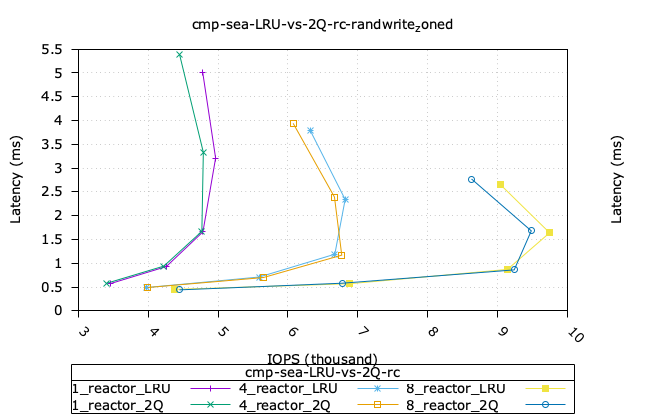
\includegraphics[width=0.8\textwidth]{../figures/cmp_sea_LRU_vs_2Q_rc_randwrite_zoned_iops_vs_lat.png}
\caption{cmp-sea-LRU-vs-2Q-rc - randwrite\_zoned}
\label{fig:cmp_sea_LRU_vs_2Q_rc_randwrite_zoned}
\end{figure}

\begin{figure}[!ht]
  \centering
  \begin{minipage}{.5\textwidth}
  \centering
    \includegraphics[width=\textwidth]{../figures/OSD_sea_1osd_1reactor_LRU_randwrite_zoned_top_cpu.png}
  \end{minipage}%
  \begin{minipage}{.5\textwidth}
  \centering
    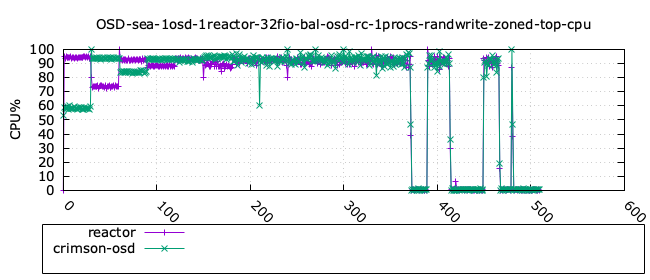
\includegraphics[width=\textwidth]{../figures/OSD_sea_1osd_1reactor_2Q_randwrite_zoned_top_cpu.png}
  \end{minipage}%
  \caption{Top CPU utilization - LRU (left) vs 2Q (right) - randwrite\_zoned, 1 reactor}
  \label{figure:1-reactor-cpu-randwrite_zoned}
\end{figure}


\begin{figure}[!ht]
  \centering
  \begin{minipage}{.5\textwidth}
  \centering
    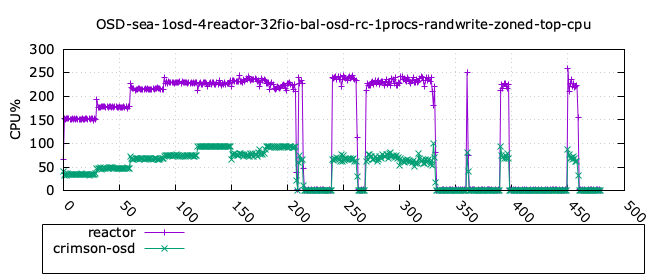
\includegraphics[width=\textwidth]{../figures/OSD_sea_1osd_4reactor_LRU_randwrite_zoned_top_cpu.png}
  \end{minipage}%
  \begin{minipage}{.5\textwidth}
  \centering
    \includegraphics[width=\textwidth]{../figures/OSD_sea_1osd_4reactor_2Q_randwrite_zoned_top_cpu.png}
  \end{minipage}%
  \caption{Top CPU utilization - LRU (left) vs 2Q (right) - randwrite\_zoned, 4 reactor}
  \label{figure:4-reactor-cpu-randwrite_zoned}
\end{figure}

\begin{figure}[!ht]
  \centering
  \begin{minipage}{.5\textwidth}
  \centering
    \includegraphics[width=\textwidth]{../figures/OSD_sea_1osd_8reactor_LRU_randwrite_zoned_top_cpu.png}
  \end{minipage}%
  \begin{minipage}{.5\textwidth}
  \centering
    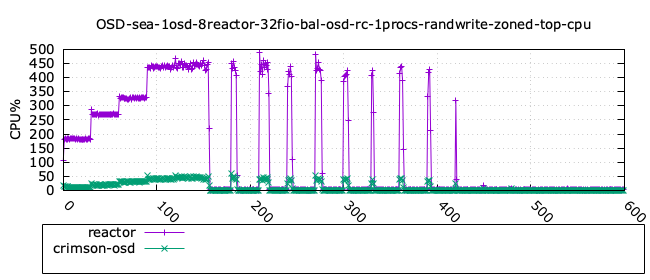
\includegraphics[width=\textwidth]{../figures/OSD_sea_1osd_8reactor_2Q_randwrite_zoned_top_cpu.png}
  \end{minipage}%
  \caption{Top CPU utilization - LRU (left) vs 2Q (right) - randwrite\_zoned, 8 reactor}
  \label{figure:8-reactor-cpu-randwrite_zoned}
\end{figure}


\pagebreak
\section{randwrite\_zipf}

This random distribution was chosen to exercise IO as follows:

\begin{verbatim}
Generating Zipf distribution with 0.768780 input and 2 GiB size and 4096 block_size.

   Rows           Hits %         Sum %           # Hits          Size
-----------------------------------------------------------------------
Top  16.67%      56.93%          56.93%           298480          1.14G
|->  33.33%      13.88%          70.81%            72775        284.28M
|->  50.00%       8.38%          79.19%            43946        171.66M
|->  66.67%       6.94%          86.13%            36364        142.05M
|->  83.33%       6.94%          93.07%            36364        142.05M
|-> 100.00%       6.93%         100.00%            36359        142.03M
-----------------------------------------------------------------------
Total                                             524288
\end{verbatim}

\begin{figure}[!ht]
\centering
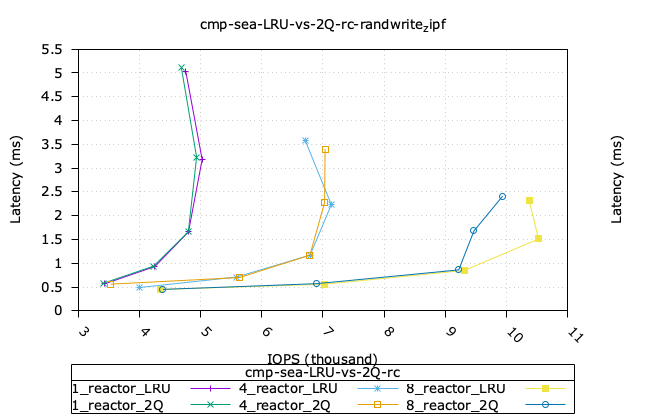
\includegraphics[width=0.8\textwidth]{../figures/cmp_sea_LRU_vs_2Q_rc_randwrite_zipf_iops_vs_lat.png}
\caption{cmp-sea-LRU-vs-2Q-rc - randwrite\_zipf}
\label{fig:cmp_sea_LRU_vs_2Q_rc_randwrite_zipf}
\end{figure}

\begin{figure}[!ht]
  \centering
  \begin{minipage}{.5\textwidth}
  \centering
    \includegraphics[width=\textwidth]{../figures/OSD_sea_1osd_1reactor_LRU_randwrite_zipf_top_cpu.png}
  \end{minipage}%
  \begin{minipage}{.5\textwidth}
  \centering
    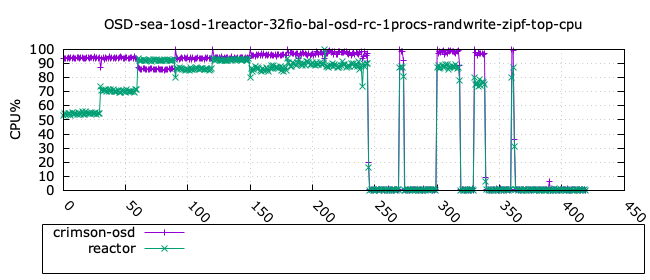
\includegraphics[width=\textwidth]{../figures/OSD_sea_1osd_1reactor_2Q_randwrite_zipf_top_cpu.png}
  \end{minipage}%
  \caption{Top CPU utilization - LRU (left) vs 2Q (right) - randwrite\_zipf, 1 reactor}
  \label{figure:1-reactor-cpu-randwrite_zipf}
\end{figure}


\begin{figure}[!ht]
  \centering
  \begin{minipage}{.5\textwidth}
  \centering
    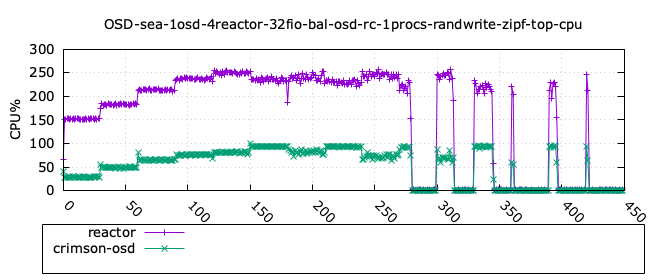
\includegraphics[width=\textwidth]{../figures/OSD_sea_1osd_4reactor_LRU_randwrite_zipf_top_cpu.png}
  \end{minipage}%
  \begin{minipage}{.5\textwidth}
  \centering
    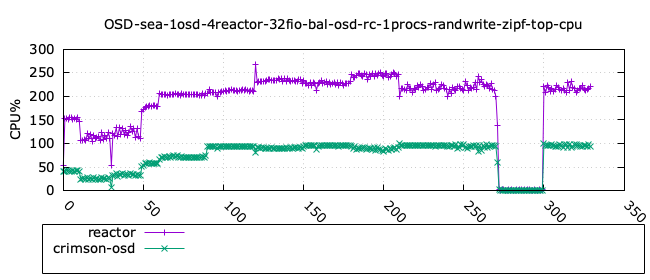
\includegraphics[width=\textwidth]{../figures/OSD_sea_1osd_4reactor_2Q_randwrite_zipf_top_cpu.png}
  \end{minipage}%
  \caption{Top CPU utilization - LRU (left) vs 2Q (right) - randwrite\_zipf, 4 reactor}
  \label{figure:4-reactor-cpu-randwrite_zipf}
\end{figure}


\begin{figure}[!ht]
  \centering
  \begin{minipage}{.5\textwidth}
  \centering
    \includegraphics[width=\textwidth]{../figures/OSD_sea_1osd_8reactor_LRU_randwrite_zipf_top_cpu.png}
  \end{minipage}%
  \begin{minipage}{.5\textwidth}
  \centering
    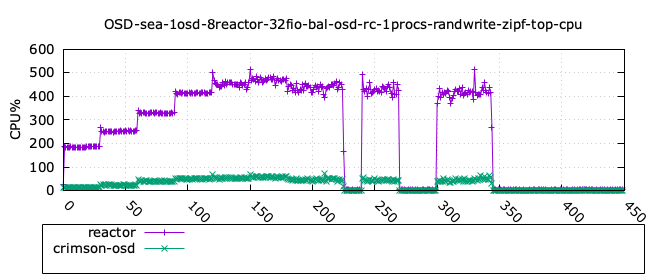
\includegraphics[width=\textwidth]{../figures/OSD_sea_1osd_8reactor_2Q_randwrite_zipf_top_cpu.png}
  \end{minipage}%
  \caption{Top CPU utilization - LRU (left) vs 2Q (right) - randwrite\_zipf, 8 reactor}
  \label{figure:8-reactor-cpu-randwrite_zipf}
\end{figure}


\pagebreak
\section{randwrite\_norm}

This is the traditional Gaussian distribution, using a generated mean and standard deviation 0.6.

\begin{figure}[!ht]
\centering
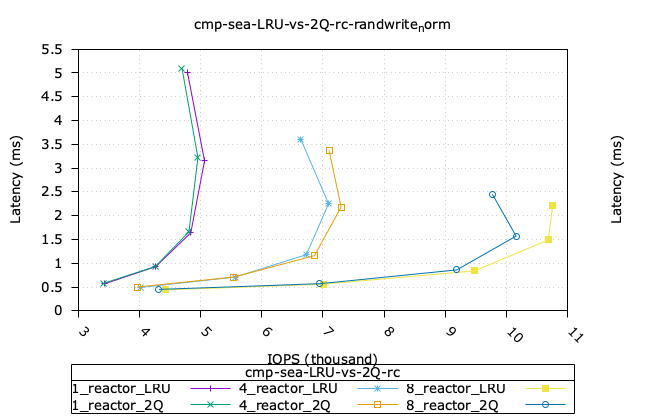
\includegraphics[width=0.8\textwidth]{../figures/cmp_sea_LRU_vs_2Q_rc_randwrite_norm_iops_vs_lat.png}
\caption{cmp-sea-LRU-vs-2Q-rc - randwrite\_norm}
\label{fig:cmp_sea_LRU_vs_2Q_rc_randwrite_norm}
\end{figure}


\begin{figure}[!ht]
  \centering
  \begin{minipage}{.5\textwidth}
  \centering
    \includegraphics[width=\textwidth]{../figures/OSD_sea_1osd_1reactor_LRU_randwrite_norm_top_cpu.png}
  \end{minipage}%
  \begin{minipage}{.5\textwidth}
  \centering
    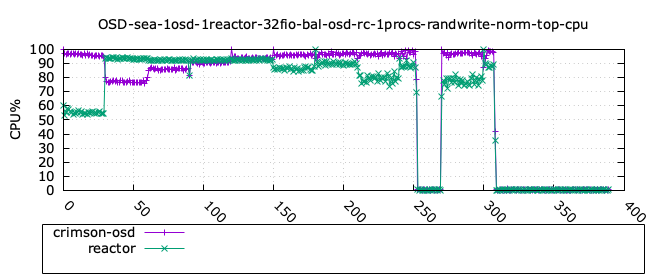
\includegraphics[width=\textwidth]{../figures/OSD_sea_1osd_1reactor_2Q_randwrite_norm_top_cpu.png}
  \end{minipage}%
  \caption{Top CPU utilization - LRU (left) vs 2Q (right) - randwrite\_norm, 1 reactor}
  \label{figure:1-reactor-cpu-randwrite_norm}
\end{figure}


\begin{figure}[!ht]
  \centering
  \begin{minipage}{.5\textwidth}
  \centering
    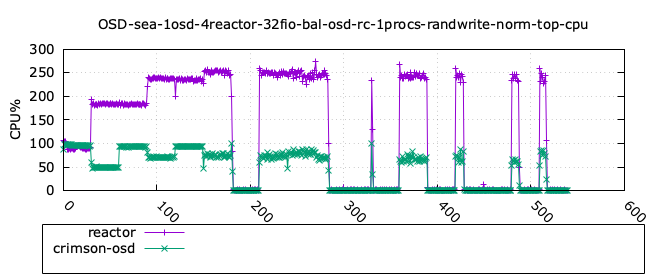
\includegraphics[width=\textwidth]{../figures/OSD_sea_1osd_4reactor_LRU_randwrite_norm_top_cpu.png}
  \end{minipage}%
  \begin{minipage}{.5\textwidth}
  \centering
    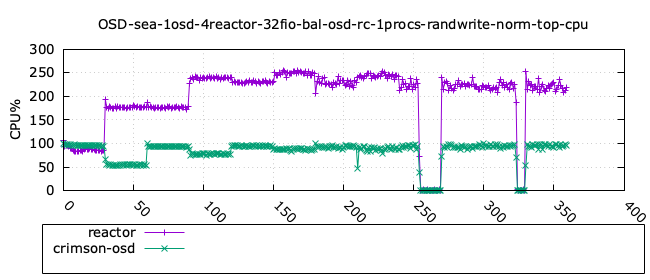
\includegraphics[width=\textwidth]{../figures/OSD_sea_1osd_4reactor_2Q_randwrite_norm_top_cpu.png}
  \end{minipage}%
  \caption{Top CPU utilization - LRU (left) vs 2Q (right) - randwrite\_norm, 4 reactor}
  \label{figure:4-reactor-cpu-randwrite_norm}
\end{figure}


\begin{figure}[!ht]
  \centering
  \begin{minipage}{.5\textwidth}
  \centering
    \includegraphics[width=\textwidth]{../figures/OSD_sea_1osd_8reactor_LRU_randwrite_norm_top_cpu.png}
  \end{minipage}%
  \begin{minipage}{.5\textwidth}
  \centering
    \includegraphics[width=\textwidth]{../figures/OSD_sea_1osd_8reactor_2Q_randwrite_norm_top_cpu.png}
  \end{minipage}%
  \caption{Top CPU utilization - LRU (left) vs 2Q (right) - randwrite\_norm, 8 reactor}
  \label{figure:8-reactor-cpu-randwrite_norm}
\end{figure}


\pagebreak
\section{randread\_zoned}

\begin{figure}[!ht]
\centering
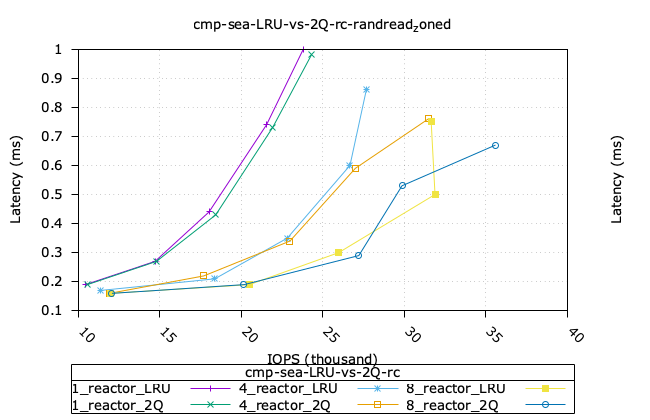
\includegraphics[width=0.8\textwidth]{../figures/cmp_sea_LRU_vs_2Q_rc_randread_zoned_iops_vs_lat.png}
\caption{cmp-sea-LRU-vs-2Q-rc - randread\_zoned}
\label{fig:cmp_sea_LRU_vs_2Q_rc_randread_zoned}
\end{figure}


\begin{figure}[!ht]
  \centering
  \begin{minipage}{.5\textwidth}
  \centering
    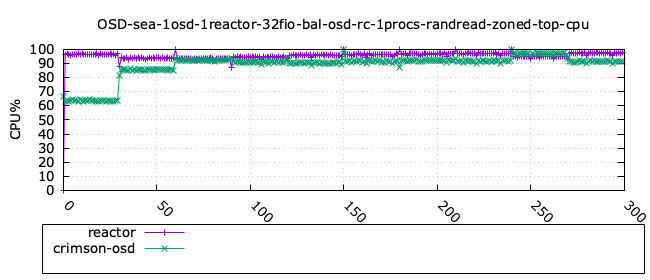
\includegraphics[width=\textwidth]{../figures/OSD_sea_1osd_1reactor_LRU_randread_zoned_top_cpu.png}
  \end{minipage}%
  \begin{minipage}{.5\textwidth}
  \centering
    \includegraphics[width=\textwidth]{../figures/OSD_sea_1osd_1reactor_2Q_randread_zoned_top_cpu.png}
  \end{minipage}%
  \caption{Top CPU utilization - LRU (left) vs 2Q (right) - randread\_zoned, 1 reactor}
  \label{figure:1-reactor-cpu-randread_zoned}
\end{figure}

\begin{figure}[!ht]
  \centering
  \begin{minipage}{.5\textwidth}
  \centering
    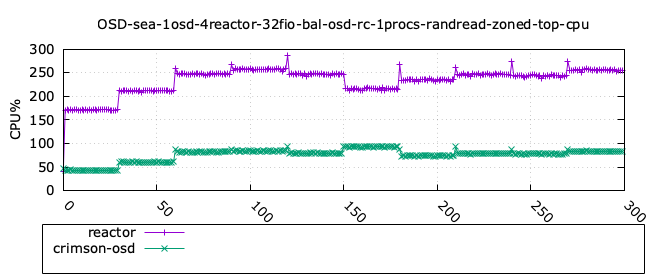
\includegraphics[width=\textwidth]{../figures/OSD_sea_1osd_4reactor_LRU_randread_zoned_top_cpu.png}
  \end{minipage}%
  \begin{minipage}{.5\textwidth}
  \centering
    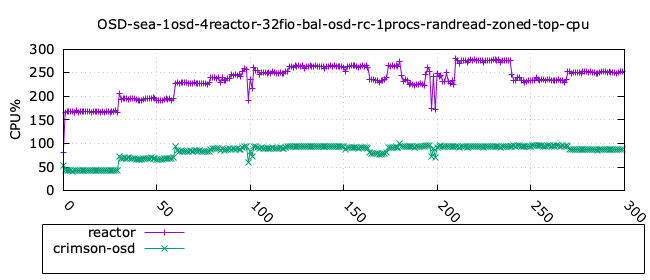
\includegraphics[width=\textwidth]{../figures/OSD_sea_1osd_4reactor_2Q_randread_zoned_top_cpu.png}
  \end{minipage}%
  \caption{Top CPU utilization - LRU (left) vs 2Q (right) - randread\_zoned, 4 reactor}
  \label{figure:4-reactor-cpu-randread_zoned}
\end{figure}

\begin{figure}[!ht]
  \centering
  \begin{minipage}{.5\textwidth}
  \centering
    \includegraphics[width=\textwidth]{../figures/OSD_sea_1osd_8reactor_LRU_randread_zoned_top_cpu.png}
  \end{minipage}%
  \begin{minipage}{.5\textwidth}
  \centering
    \includegraphics[width=\textwidth]{../figures/OSD_sea_1osd_8reactor_2Q_randread_zoned_top_cpu.png}
  \end{minipage}%
  \caption{Top CPU utilization - LRU (left) vs 2Q (right) - randread\_zoned, 8 reactor}
  \label{figure:8-reactor-cpu-randread_zoned}
\end{figure}

\pagebreak
\section{randread\_zipf}

\begin{figure}[!ht]
\centering
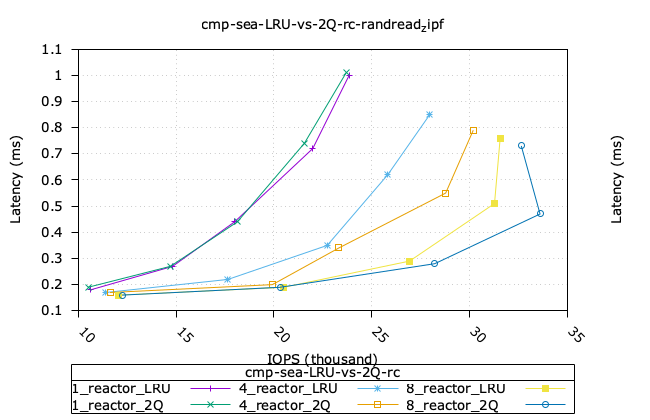
\includegraphics[width=0.8\textwidth]{../figures/cmp_sea_LRU_vs_2Q_rc_randread_zipf_iops_vs_lat.png}
\caption{cmp-sea-LRU-vs-2Q-rc - randread\_zipf}
\label{fig:cmp_sea_LRU_vs_2Q_rc_randread_zipf}
\end{figure}


\begin{figure}[!ht]
  \centering
  \begin{minipage}{.5\textwidth}
  \centering
    \includegraphics[width=\textwidth]{../figures/OSD_sea_1osd_1reactor_LRU_randread_zipf_top_cpu.png}
  \end{minipage}%
  \begin{minipage}{.5\textwidth}
  \centering
    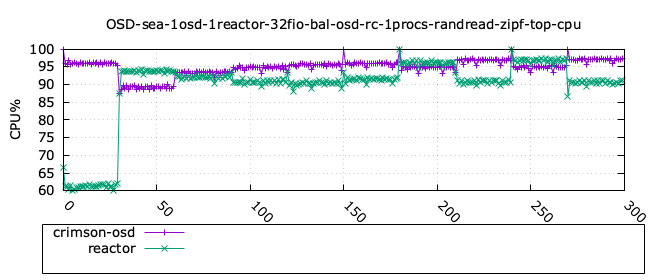
\includegraphics[width=\textwidth]{../figures/OSD_sea_1osd_1reactor_2Q_randread_zipf_top_cpu.png}
  \end{minipage}%
  \caption{Top CPU utilization - LRU (left) vs 2Q (right) - randread\_zipf, 1 reactor}
  \label{figure:1-reactor-cpu-randread_zipf}
\end{figure}


\begin{figure}[!ht]
  \centering
  \begin{minipage}{.5\textwidth}
  \centering
    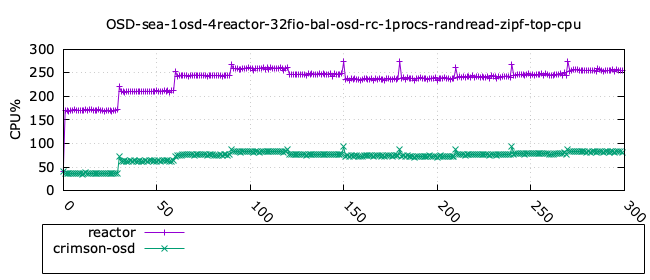
\includegraphics[width=\textwidth]{../figures/OSD_sea_1osd_4reactor_LRU_randread_zipf_top_cpu.png}
  \end{minipage}%
  \begin{minipage}{.5\textwidth}
  \centering
    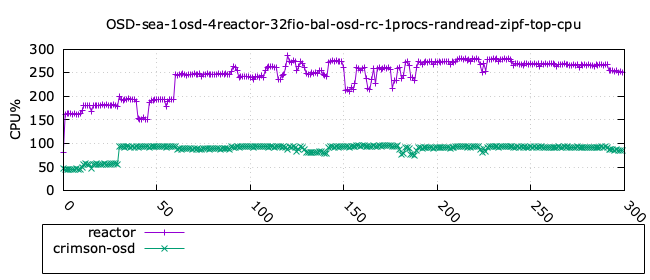
\includegraphics[width=\textwidth]{../figures/OSD_sea_1osd_4reactor_2Q_randread_zipf_top_cpu.png}
  \end{minipage}%
  \caption{Top CPU utilization - LRU (left) vs 2Q (right) - randread\_zipf, 4 reactor}
  \label{figure:4-reactor-cpu-randread_zipf}
\end{figure}


\begin{figure}[!ht]
  \centering
  \begin{minipage}{.5\textwidth}
  \centering
    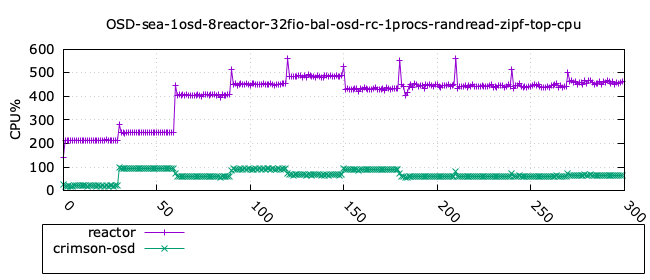
\includegraphics[width=\textwidth]{../figures/OSD_sea_1osd_8reactor_LRU_randread_zipf_top_cpu.png}
  \end{minipage}%
  \begin{minipage}{.5\textwidth}
  \centering
    \includegraphics[width=\textwidth]{../figures/OSD_sea_1osd_8reactor_2Q_randread_zipf_top_cpu.png}
  \end{minipage}%
  \caption{Top CPU utilization - LRU (left) vs 2Q (right) - randread\_zipf, 8 reactor}
  \label{figure:8-reactor-cpu-randread_zipf}
\end{figure}


\pagebreak
\section{randread\_norm}

\begin{figure}[!ht]
\centering
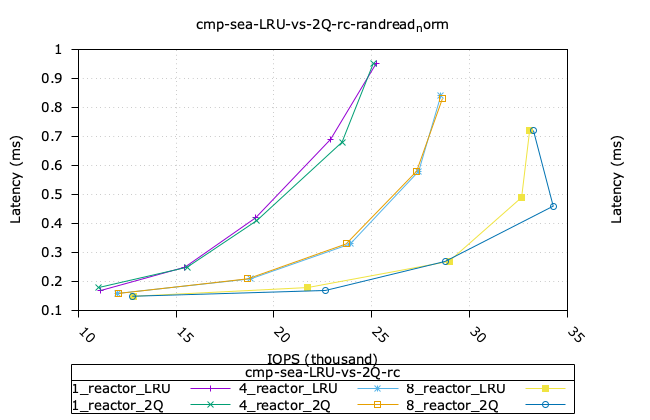
\includegraphics[width=0.8\textwidth]{../figures/cmp_sea_LRU_vs_2Q_rc_randread_norm_iops_vs_lat.png}
\caption{cmp-sea-LRU-vs-2Q-rc - randread\_norm}
\label{fig:cmp_sea_LRU_vs_2Q_rc_randread_norm}
\end{figure}

\begin{figure}[!ht]
  \centering
  \begin{minipage}{.5\textwidth}
  \centering
    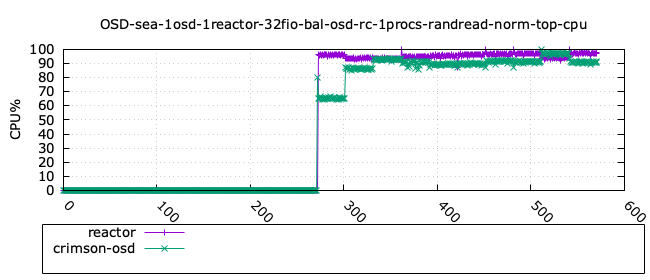
\includegraphics[width=\textwidth]{../figures/OSD_sea_1osd_1reactor_LRU_randread_norm_top_cpu.png}
  \end{minipage}%
  \begin{minipage}{.5\textwidth}
  \centering
    \includegraphics[width=\textwidth]{../figures/OSD_sea_1osd_1reactor_2Q_randread_norm_top_cpu.png}
  \end{minipage}%
  \caption{Top CPU utilization - LRU (left) vs 2Q (right) - randread\_norm, 1 reactor}
  \label{figure:1-reactor-cpu-randread_norm}
\end{figure}


\begin{figure}[!ht]
  \centering
  \begin{minipage}{.5\textwidth}
  \centering
    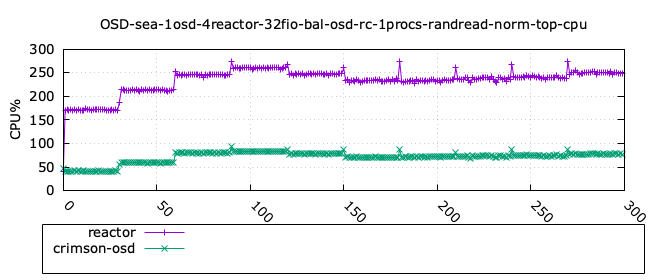
\includegraphics[width=\textwidth]{../figures/OSD_sea_1osd_4reactor_LRU_randread_norm_top_cpu.png}
  \end{minipage}%
  \begin{minipage}{.5\textwidth}
  \centering
    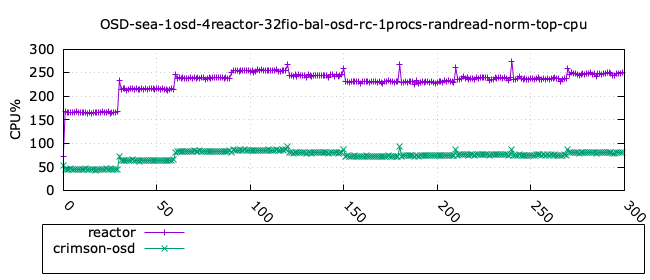
\includegraphics[width=\textwidth]{../figures/OSD_sea_1osd_4reactor_2Q_randread_norm_top_cpu.png}
  \end{minipage}%
  \caption{Top CPU utilization - LRU (left) vs 2Q (right) - randread\_norm, 4 reactor}
  \label{figure:4-reactor-cpu-randread_norm}
\end{figure}


\begin{figure}[!ht]
  \centering
  \begin{minipage}{.5\textwidth}
  \centering
    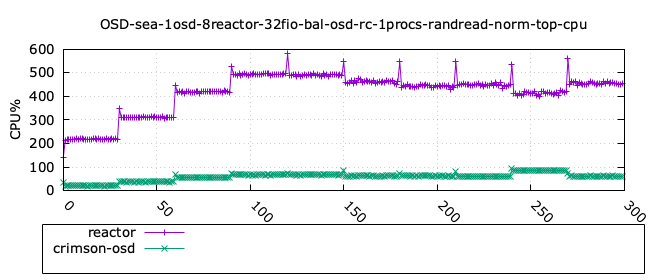
\includegraphics[width=\textwidth]{../figures/OSD_sea_1osd_8reactor_LRU_randread_norm_top_cpu.png}
  \end{minipage}%
  \begin{minipage}{.5\textwidth}
  \centering
    \includegraphics[width=\textwidth]{../figures/OSD_sea_1osd_8reactor_2Q_randread_norm_top_cpu.png}
  \end{minipage}%
  \caption{Top CPU utilization - LRU (left) vs 2Q (right) - randread\_norm, 8 reactor}
  \label{figure:8-reactor-cpu-randread_norm}
\end{figure}


\clearpage

\appendix
%\input{configuration}
%\input{estimation}

\end{document}
%%%%%%%%%%%%%%%%%%%%%%%%%%%%%%

